\section{Relation to flip-reachability logic}\label{sec:freach}


In this section we prove \Cref{thm:main-freach}. The main part of the work is presented in \cref{sec:low-rank-comb}, where we develop a combinatorial characterization of sets of low rank in undirected graphs. This description is captured in the key technical statement: Low Rank Structure Theorem (\cref{thm:low-rank-structure}). Then, we complete the proof of \Cref{thm:main-freach} in \cref{sec:flip-reach-proof}.


\subsection{Combinatorics of sets of low rank}
\label{sec:low-rank-comb}

For an undirected graph $G$ and $r \in \N$, we define $\LowRank^r(G)$ to be the family of all vertex sets in $G$ of rank at most $r$:
\[
    \LowRank^r(G) \coloneqq \{ X \subseteq V(G) \,\mid\, \rk(X) \leq r \}.
\]
Our main goal in this section is to give an~effective representation of $\LowRank^r(G)$.
More precisely, we will show that $\LowRank^r(G)$ can be written as the~union of $|V(G)|^{\Oh_r(1)}$ \emph{well-structured} families of subsets of $V(G)$, and that each such family can be defined using $\Oh_r(1)$ vertices of $G$.
Formal definitions follow.

Let $G$ be an~undirected graph.
A~\emph{seed} of $G$ is a~tuple $(X_+, X_-, \Xc)$, where
\begin{itemize}[nosep]
 \item $X_+, X_- \subseteq V(G)$,
 \item $\Xc$ is a~collection of nonempty subsets of $V(G)$ (called {\em{parts}}), and
 \item $\Xc \cup \{X_+, X_-\}$ is a~partition of $V(G)$.
\end{itemize}
The family \emph{spanned} by a~seed $(X_+, X_-, \Xc)$ is
\[ \Span(X_+, X_-, \Xc) \coloneqq \{X_+ \cup \, \bigcup \mathcal{Y} \,\colon\, \mathcal{Y} \subseteq \Xc\}. \]
In our characterization of  $\mathsf{LowRank}^r(G)$, the obtained families covering  $\mathsf{LowRank}^r(G)$ can be spanned by seeds with two additional structural restrictions: first, they need to satisfy a~specific uniformity condition, which we will introduce in a~moment; and second, the seeds themselves need to be defined in terms of at most $\Oh_r(1)$ vertices of $G$ via fixed formulas of flip-reachability logic.

For any seed $(X_+, X_-, \Xc)$ and $u \in \bigcup \Xc$, we define $\Xc(u) \in \Xc$ as the unique part of $\Xc$ containing $u$.
Then, given a~tuple $\tup{a}$ of vertices of $G$, we say that a~seed $(X_+, X_-, \Xc)$ is \emph{$\tup{a}$-uniform} if for every $u_1, u_2 \in \bigcup \Xc$ with $\atp(u_1, \tup{a}) = \atp(u_2, \tup{a})$, we have that $N_G(u_1) \setminus (\Xc(u_1) \cup \Xc(u_2)) = N_G(u_2) \setminus (\Xc(u_1) \cup \Xc(u_2))$.
In other words, whenever $u_1$ and $u_2$ are twins with respect to $\tup{a}$, they are also twins with respect to $V(G) \setminus (\Xc(u_1) \cup \Xc(u_2))$.

Next, we say that a~seed $(X_+, X_-, \Xc)$ is \emph{defined} by formulas $\varphi_+$, $\varphi_-$, $\varphi_{\sim}$ of flip-reachability logic and a~$k$-tuple of vertices $\tup{a}$ if:
\begin{itemize}[nosep]
    \item $X_+ = \{v \in V(G) \,\colon\, G \models \varphi_+(v, \tup{a})\}$,
    \item $X_- = \{v \in V(G) \,\colon\, G \models \varphi_-(v, \tup{a})\}$, and
    \item two vertices $u, v \in V(G) \setminus (X_+ \cup X_-)$ belong to the same part of $\Xc$ if and only if $G \models \varphi_\sim(u, v, \tup{a})$.
\end{itemize}
Note that, assuming that $\varphi_+(\cdot, \tup{a})$ and $\varphi_-(\cdot, \tup{a})$ describe disjoint subsets of $V(G)$ and $\varphi_{\sim}(\cdot, \cdot, \tup{a})$ is an~equivalence relation on $V(G)$, there exists a~unique seed defined by $\varphi_+, \varphi_-, \varphi_{\sim}$ and $\tup{a}$.
We denote this seed by $\Seed(\varphi_+, \varphi_-, \varphi_{\sim}, \tup{a})$.

We are now ready to state our structural characterization of vertex sets of bounded rank.
\begin{theorem}[Low Rank Structure Theorem]
    \label{thm:low-rank-structure}
    Let $r \in \N$.
    Then there exist an~integer $k \coloneqq k(r)$ and formulas $\varphi_+$, $\varphi_-$, $\varphi_{\sim}$ of flip-reachability logic with the following properties:
    \begin{itemize}[nosep]
        \item For any undirected graph $G$ and $k$-tuple $\tup{a} \in V(G)^k$, we have that $\varphi_+, \varphi_-, \varphi_{\sim}, \tup{a}$ define an~$\tup{a}$-uniform seed of $G$.
        \item For any undirected graph $G$,
        \[
            \LowRank^r(G) = \bigcup_{\tup{a} \in V(G)^k} \Span(\Seed(\varphi_+, \varphi_-, \varphi_{\sim}, \tup{a})).
        \]
    \end{itemize}
\end{theorem}

The remainder of this section is devoted to the proof of the Low Rank Structure Theorem (\cref{thm:low-rank-structure}).


\subsubsection{Sets of low rank described as suffixes of flips}

As the first step towards the proof of \cref{thm:low-rank-structure}, we show that the family of low-rank vertex sets in $G$ can be characterized as \emph{suffixes} of certain digraphs that are flips of $G$ parameterized by a~bounded number of vertices.
Namely, our goal is to prove the following statement:

\begin{lemma}
    \label{lem:low-rank-to-suffixes}
    Let $r \in \N$.
    Then there exist an~integer $k \coloneqq k(r)$ and a~binary relation $A \subseteq \atp^{k+1} \times \atp^{k+1}$ such that, for any undirected graph $G$, we have
    \[
        \LowRank^r(G) = \bigcup_{\tup{a} \in V(G)^k} \Suffixes(G \oplus_{\tup{a}} A),
    \]
    where $\Suffixes(H)$ denotes the set of suffixes of a~directed graph $H$: \[\Suffixes(H) \coloneqq \{S \subseteq V(H) \,\colon\, \forall_{\vec{uv} \in E(H)}\, u \in S \Rightarrow v \in S\}.\]
\end{lemma}

The proof of \Cref{lem:low-rank-to-suffixes} will roughly proceed as follows.
Suppose $G$ is an~undirected graph.
Given a~set $S \subseteq V(G)$, we say that its subset $R_S \subseteq S$ is a~\emph{representative} of $S$ if every vertex $v \in S \setminus R_S$ has a~twin $r_v \in R_S$ with respect to $V(G) \setminus S$.
Equivalently,
\[
    \{ N(v) \setminus S \,\colon\, v \in R_S \} \,=\, \{ N(v) \setminus S \,\colon\, v \in S \}.
\]
Let now $X \subseteq V(G)$ be a set of vertices of rank at most $r$.
We invoke the following standard fact:
\begin{proposition}[\cite{OumS06}]
    \label{prop:small-representative}
    There exists a~representative $R_+$ of $X$ of cardinality at most $2^r$, as well as a~representative $R_-$ of $V(G) \setminus X$ of cardinality at most $2^r$.
\end{proposition}
So let us choose the representatives $R_+, R_-$ as above, and assume that these are inclusionwise minimal.
Our aim is now to recover $X$ given $R_+$ and $R_-$; or more precisely, find all possible sets $X \subseteq V(G)$ with $R_+$ forming a~representative of $X$ and $R_-$ forming a~representative of $V(G) \setminus X$.
To this aim, observe that every vertex $v \in V(G)$ has at most one twin $r_v^+ \in R_+$ with respect to $V(G) \setminus X$ (and such a~twin definitely exists when $v \in X$), and similarly, $v$ has at most one twin $r_v^- \in R_-$ with respect to $X$ (and it exists whenever $v \notin X$).
We can now easily reason about some of the vertices in $G$: for instance, a~vertex $v$ must belong to $X$ if $v \in R_+$ or $v$ has no twin in $R_-$ with respect to $X$; and $v$ must not belong to $X$ if $v \in R_-$ or $v$ has no twin in $R_+$ with respect to $V(G) \setminus X$.
What happens with the remaining vertices is a~bit trickier: we will show that there exists a~flip $H \coloneqq G \oplus_{\tup{a}} A$, with $\tup{a}$ consisting precisely of the vertices of $R_+ \cup R_-$, with the property that whenever $\vec{uv}$ is an~arc of $H$, then $u \in X$ implies $v \in X$.
The precise details follow below.

\medskip

We begin by explaining the construction of the flip $G \oplus_{\tup{a}} A$.
Fix $r \in \N$ for the course of the proof and set $k \coloneqq 2 \cdot 2^r$.
We consider every $k$-tuple $\tup{a} \in V(G)^k$ of parameters to consist of two halves $\tup{a}^+ = (a^+_1, \ldots, a^+_{2^r})$, $\tup{a}^- = (a^-_1, \ldots, a^-_{2^r})$; intuitively, for a~low-rank subset $X$ of $V(G)$, $\tup{a}^+$ denotes a~representative set of $X$ with respect to $V(G) \setminus X$, and $\tup{a}^-$ denotes a~representative set of $V(G) \setminus X$ with respect to $X$.
In the following description, we will often slightly abuse the notation and use $\tup{a}^+$ and $\tup{a}^-$ to denote the set of vertices present in the respective tuple of vertices.

For every $v \in V(G)$, we can deduce from the atomic type $\atp(v, \tup{a}^+, \tup{a}^-) \in \atp^{k+1}$ in $G$ the following information:
\begin{itemize}[nosep]
    \item whether $\tup{a}^+$ and $\tup{a}^-$ are disjoint;
    \item the subgraph $G[\tup{a}]$ of $G$ induced by $\tup{a}$;
    \item whether in $G[\tup{a}]$, the set $\tup{a}^+$ of vertices has rank at most $k$;
    \item whether $v \in \tup{a}^+$ and whether $v \in \tup{a}^-$;
    \item a~vertex $\varphi^+(v) \in \tup{a}^+$ with the property that $N(v) \cap \tup{a}^- = N(\varphi^+(v)) \cap \tup{a}^-$; we place $\varphi^+(v) = \bot$ if no such vertex exists, and in case multiple such vertices exist, we choose $\varphi^+(v)$ as the earliest entry of $\tup{a}^+$ with this property;
    \item an~analogous vertex $\varphi^-(v) \in \tup{a}^-$ with the property that $N(v) \cap \tup{a}^+ = N(\varphi^-(v)) \cap \tup{a}^+$ (again, we place $\varphi^-(v) = \bot$ if no such vertex exists).
\end{itemize}
Following the intuition above, assume that $X$ is a~low-rank subset of $V(G)$ and let $v \in V(G)$.
If $v \in X$, then $\varphi^+(v)$ specifies the twin of $v$ in $X$ with respect to $V(G) \setminus X$; and conversely, if $v \notin X$, then $\varphi^-(v)$ denotes the twin of $v$ in $V(G) \setminus X$ with respect to $X$.
In particular, $\varphi^+(v) = \bot$ implies that $v \notin X$, and $\varphi^-(v) = \bot$ implies that $v \in X$.
Also, $\varphi^+(v) \neq \bot$ implies that $\varphi^+(\varphi^+(v)) = \varphi^+(v)$ and similarly $\varphi^-(v) \neq \bot$ implies that $\varphi^-(\varphi^-(v)) = \varphi^-(v)$.

Now, given a~graph $G$ and a~tuple $\tup{a} \in V(G)^k$, we construct the~digraph $H_{\tup{a}} = (V, E_{\tup{a}})$ as follows.
We say that a~tuple $\tup{a}$ is \emph{admissible} if $\tup{a}^+$ and $\tup{a}^-$ are disjoint and in $G[\tup{a}]$, the set $\tup{a}^+$ of vertices has rank at most~$r$; the tuple is \emph{inadmissible} otherwise.
If $\tup{a}$ is inadmissible, we specify that $\vec{uv}$ is an~arc of $H_{\tup{a}}$ if at least one of the endpoints of the arc belongs to $\tup{a}$ or $uv$ is an~edge of $G$.
On the other hand, if $\tup{a}$ is admissible, we specify that $\vec{uv}$ is an~arc of $H_{\tup{a}}$ if any of the following conditions hold:
\begin{enumerate}[(i),nosep]
    \item \label{item:cond-is-param} $u \in \tup{a}^-$ or $v \in \tup{a}^+$;
    \item \label{item:cond-must-be-minus} $\varphi^+(u) = \bot$ and $v \in \tup{a}^-$;
    \item \label{item:cond-must-be-plus} $u \in \tup{a}^+$ and $\varphi^-(v) = \bot$;
    \item \label{item:cond-general} $E(u, v)\ \textrm{xor}\ [\varphi^+(u) \neq \bot\ \textrm{and}\ \varphi^-(v) \neq \bot \ \textrm{and}\ E(\varphi^+(u), \varphi^-(v))]$.
\end{enumerate}


Intuitively, condition \ref{item:cond-is-param} ensures that whenever $X$ is a~non-trivial suffix of $H_{\tup{a}}$ (i.e., a~suffix different from $\emptyset$ and $V(G)$), we necessarily have $\tup{a}^- \cap X = \emptyset$ and $\tup{a}^+ \subseteq X$.
Then conditions \ref{item:cond-must-be-minus}, \ref{item:cond-must-be-plus} ensure that $u \notin X$ whenever $\varphi^+(u) = \bot$ and $v \in X$ whenever $\varphi^-(v) = \bot$, respectively.
Finally, \ref{item:cond-general} will resolve the general case, encoding all possible implications of the form ``if some vertex $u$ belongs to $X$, then another vertex $v$ belongs to $X$ as well''.

\begin{example}
    Consider the graph $G$ from \Cref{sfig:dir-flip-example-before}, with $\tup{a}^- = (a^-_1, a^-_2)$ and $a^+ = (a^+_1, a^+_2)$.
    We have:
    \begin{center}
        \begin{tabular}{|c||c|c|c|c|c|c|c|c|}
            \hline
            $\mathbf{w}$ & $a^-_1$ & $a^-_2$ & $a^+_1$ & $a^+_2$ & $w_1$ & $w_2$ & $w_3$ & $w_4$ \\ \hline \hline
            $\mathbf{\varphi^+(w)}$ & $\bot$ & $\bot$ & $a^+_1$ & $a^+_2$ & $\bot$ & $a^+_1$ & $a^+_2$ & $a^+_2$ \\ \hline
            $\mathbf{\varphi^-(w)}$ & $a^-_1$ & $a^-_2$ & $\bot$ & $\bot$ & $a^-_1$ & $a^-_1$ & $a^-_1$ & $\bot$ \\ \hline
        \end{tabular}
    \end{center}
    The corresponding digraph $H_{\tup{a}}$ is given in \Cref{sfig:dir-flip-example-after}.

    Black arcs are of type \ref{item:cond-is-param}; these ensure that every non-trivial suffix of $H_{\tup{a}}$ contains $a^+_1, a^+_2$ and does not contain $a^-_1, a^-_2$.

    Since $\varphi^+(w_1) = \bot$ (so $w_1$ cannot belong to $X$), we additionally introduce arcs of type \ref{item:cond-must-be-minus} (blue), warranting that non-trivial suffixes of $H_{\tup{a}}$ do not contain $w_1$.

    Since $\varphi^-(w_4) = \bot$ (so $w_4$ must belong to $X$), we add arcs of type \ref{item:cond-must-be-plus} (yellow), ensuring that non-trivial suffixes of $H_{\tup{a}}$ contain $w_4$.

    Observe that $w_2w_3$ is a~non-edge in $G$, but $\varphi^+(w_2) \varphi^-(w_3)$ is an~edge in $G$.
    Therefore it cannot be that $w_2 \in X$ and $w_3 \notin X$: the statement $w_2 \in X$ implies that $\varphi^+(w_2)$ is a~twin of $w_2$ with respect to $V(G) \setminus X$, and the statement $w_3 \notin X$ implies that $\varphi^-(w_3)$ is a~twin of $w_3$ with respect to $X$.
    The (pink) arc $\vec{w_2w_3}$ in $H_{\tup{a}}$ of type \ref{item:cond-general} encodes this dependency: every suffix of $H_{\tup{a}}$ containing $w_2$ must also contain $w_3$.

    The non-trivial suffixes of $H_{\tup{a}}$ are $\{a^+_1, a^+_2, w_4\}$, $\{a^+_1, a^+_2, w_3, w_4\}$ and $\{a^+_1, a^+_2, w_2, w_3, w_4\}$.
    It can be verified that those are precisely the sets $X$ for which $\{a^+_1, a^+_2\}$ is a~representative of $X$ and $\{a^-_1, a^-_2\}$ is a~representative of $V(G) \setminus X$.
    
    \begin{figure}[ht]
        \begin{subfigure}[t]{0.5\textwidth}
            \centering
            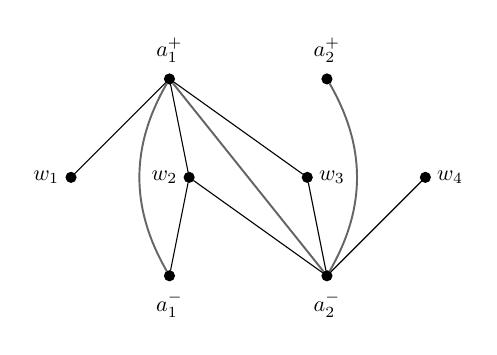
\begin{tikzpicture}[every node/.style={draw, circle, scale=0.8, thick,fill=black,inner sep=1.4}]
                \node[label=180:$w_1$] (w1) at (-2.25,0) {};
                \node[label=180:$w_2$] (w2) at (-0.75,0) {};
                \node[label=0:$w_3$] (w3) at (0.75,0) {};
                \node[label=0:$w_4$] (w4) at (2.25,0) {};

                \node[label=90:$a_1^+$] (a1p) at (-1,1.25) {};
                \node[label=90:$a_2^+$] (a2p) at (1,1.25) {};
                \node[label=-90:$a_1^-$] (a1m) at (-1,-1.25) {};
                \node[label=-90:$a_2^-$] (a2m) at (1,-1.25) {};

                \draw (a1p) to (w1) (a1p) to (w2) (a1p) to (w3);
                \draw (a1m) to (w2) (a2m) to (w2) (a2m) to (w3) (a2m) to (w4);
                \draw[line width=0.7pt,black!60!white] (a1p) [bend right=30] to (a1m) (a1p) [bend right=0] to (a2m) (a2p) [bend left=30] to (a2m);
            \end{tikzpicture}   
            \caption{Graph $G$.}
            \label{sfig:dir-flip-example-before}
        \end{subfigure}%
        \begin{subfigure}[t]{0.5\textwidth}
            \centering
            \begin{tikzpicture}[every node/.style={draw, circle, scale=0.8, thick,fill=black,inner sep=1.4}]
                \node[label=180:$w_1$] (w1) at (-2.25,0) {};
                \node[label=180:$w_2$] (w2) at (-0.75,0) {};
                \node[label=0:$w_3$] (w3) at (0.75,0) {};
                \node[label=0:$w_4$] (w4) at (2.25,0) {};

                \node[label=90:$a_1^+$] (a1p) at (-1,1.25) {};
                \node[label=90:$a_2^+$] (a2p) at (1,1.25) {};
                \node[label=-90:$a_1^-$] (a1m) at (-1,-1.25) {};
                \node[label=-90:$a_2^-$] (a2m) at (1,-1.25) {};

                %arcs to a plus
                \draw[arrows = {-Latex[width=0pt 7, length=5pt]}] (w1) [bend right= 10] to (a1p);
                \draw[arrows = {-Latex[width=0pt 7, length=5pt]}]  (w1) [bend right= 15] to (a2p);
                \draw[arrows = {-Latex[width=0pt 7, length=5pt]}] (w2) [bend left= 15] to (a1p);
                \draw[arrows = {-Latex[width=0pt 7, length=5pt]}]  (w2) [bend right= 27] to (a2p);
                \draw[arrows = {-Latex[width=0pt 7, length=5pt]}] (w3) [bend left= 27] to (a1p);
                \draw[arrows = {-Latex[width=0pt 7, length=5pt]}]  (w3) [bend right= 15] to (a2p);
                \draw[arrows = {-Latex[width=0pt 7, length=5pt]}] (w4) [bend left= 15] to (a1p);
                \draw[arrows = {-Latex[width=0pt 7, length=5pt]}]  (w4) [bend left= 10] to (a2p);
                \draw[arrows = {-Latex[width=0pt 7, length=5pt]}]  (a1p) [bend left= 10] to (a2p);
                \draw[arrows = {-Latex[width=0pt 7, length=5pt]}]  (a2p) [bend left= 10] to (a1p);

                %arcs from a minus
                \draw[arrows = {-Latex[width=0pt 7, length=5pt]}] (a1m) [bend right= 10] to (w1);
                \draw[arrows = {-Latex[width=0pt 7, length=5pt]}]  (a2m) [bend right= 15] to (w1);
                \draw[arrows = {-Latex[width=0pt 7, length=5pt]}] (a1m) [bend left= 15] to (w2);
                \draw[arrows = {-Latex[width=0pt 7, length=5pt]}]  (a2m) [bend right= 5] to (w2);
                \draw[arrows = {-Latex[width=0pt 7, length=5pt]}] (a1m) [bend left= 5] to (w3);
                \draw[arrows = {-Latex[width=0pt 7, length=5pt]}]  (a2m) [bend right= 15] to (w3);
                \draw[arrows = {-Latex[width=0pt 7, length=5pt]}] (a1m) [bend left= 15] to (w4);
                \draw[arrows = {-Latex[width=0pt 7, length=5pt]}]  (a2m) [bend left= 10] to (w4);
                \draw[arrows = {-Latex[width=0pt 7, length=5pt]}]  (a1m) [bend right= 15] to (a2m);
                \draw[arrows = {-Latex[width=0pt 7, length=5pt]}]  (a2m) [bend right= 5] to (a1m);

                \draw[line width=0.5pt,custom-pink,arrows = {-Latex[width=0pt 7, length=5pt]}]  (w2) [bend right= 5] to (w3);

                %extra arcs
                \draw[line width=0.5pt,custom-blue,arrows = {-Latex[width=0pt 7, length=5pt]}]  (w1) [bend right= 10] to (a1m);
                \draw[line width=0.5pt,custom-blue,arrows = {-Latex[width=0pt 7, length=5pt]}]  (w1) [bend right= 0] to (a2m);
                \draw[line width=0.5pt,custom-orange,arrows = {-Latex[width=0pt 7, length=5pt]}]  (a1p) [bend left= 0] to (w4);
                \draw[line width=0.5pt,custom-orange,arrows = {-Latex[width=0pt 7, length=5pt]}]  (a2p) [bend left= 10] to (w4);
            \end{tikzpicture}
            \caption{Digraph $H_{\tup{a}}$.}
            \label{sfig:dir-flip-example-after}
        \end{subfigure}
        \caption{Example graph $G$ and construction of the~digraph $H_{\tup{a}}$ from an~admissible tuple $\tup{a}$.}
        \label{fig:dir-flip-example}
    \end{figure}
\end{example}

We first show that $H_{\tup{a}}$ is indeed a~flip of $G$ with parameters $\tup{a}$:

\begin{lemma}
    \label{lem:low-rank-to-suffixes-exists-relation}
    There exists a~binary relation $A \subseteq \atp^{k+1} \times \atp^{k+1}$ such that, for any undirected graph $G$ and any tuple $\tup{a} \in V(G)^k$, we have $H_{\tup{a}} = G \oplus_{\tup{a}} A$.
\end{lemma}
\begin{proof}
    Let $\tau_u, \tau_v \in \atp^{k+1}$.
    We need to prove that for any undirected graph $G$, any $k$-tuple $\tup{a}$ and any pair of distinct vertices $u, v \in V(G)$ with $\atp(u, \tup{a}) = \tau_u$, $\atp(v, \tup{a}) = \tau_v$, the value $\lambda_{\tup{a}}(u, v) \coloneqq E_{\tup{a}}(u, v)\ \textrm{xor}\ E(u, v)$ depends only on the pair of types $(\tau_u, \tau_v)$.
    Hence choose $G$, $\tup{a}$, $u$ and $v$ as above.

    From $\tau_u$ (and analogously from $\tau_v$) we can deduce whether $\tup{a}$ is admissible.
    First, suppose that $\tup{a}$ is inadmissible.
    If $u \in \tup{a}$ (which can be deduced from $\tau_u$), then we have $(u, v) \in E_{\tup{a}}$, so the value $\lambda_{\tup{a}}(u, v) = E_{\tup{a}}(u, v) \ \textrm{xor}\ E(u, v) = \neg E(u, v)$ is uniquely implied by $\tau_v$ (since $u \in \tup{a}$ and the atomic type $\tau_v$ determines $N(v) \cap \tup{a}$).
    Symmetrically, if $v \in \tup{a}$, then $\lambda_{\tup{a}}(u, v)$ can be deduced from $\tau_u$.
    On the other hand, if $u, v \notin \tup{a}$, then $\lambda_{\tup{a}}(u, v)$ is simply false, so it is enough to specify that $(\tau_u, \tau_v) \notin A$.

    Now consider the case when $\tup{a}$ is admissible.
    The satisfaction of any of the conditions \ref{item:cond-is-param}, \ref{item:cond-must-be-minus}, \ref{item:cond-must-be-plus} can be verified by examining the atomic types $\tau_u$ and $\tau_v$.
    In each of these cases, we have $\lambda_{\tup{a}}(u, v) = \neg E(u, v)$, and the value $E(u, v)$ is uniquely determined by $\tau_u$ (if $v \in \tup{a}$) or by $\tau_v$ (if $u \in \tup{a}$).
    On the other hand, if none of these cases hold, then the value $\lambda_{\tup{a}}(u, v) = [\varphi^+(u) \neq \bot\ \textrm{and}\ \varphi^-(v) \neq \bot\ \textrm{and}\ E(\varphi^+(u), \varphi^-(v))]$ can be inferred from the pair $(\tau_u, \tau_v)$.
\end{proof}

It remains to show that the family of subsets of $V(G)$ of rank at most $r$ is equivalent to the family of suffixes of the graphs $H_{\tup{a}}$.
We prove each implication of this equivalence separately. First we  argue that each suffix of $H_{\tup{a}}$ indeed has small rank.

\begin{lemma}
    \label{lem:low-rank-to-suffixes-rtl}
    Let $G$ be an~undirected graph, $\tup{a} \in V(G)^k$ and $X \in \Suffixes(H_{\tup{a}})$.
    Then $\rk(X) \leq r$.
\end{lemma}
\begin{proof}
    If $\tup{a}$ is inadmissible, then $H_{\tup{a}}$ is undirected and every vertex $v \in \tup{a}$ is a~universal vertex of $H_{\tup{a}}$.
    In particular, $\Suffixes(H_{\tup{a}}) = \{\emptyset, V(G)\}$ and the lemma holds.
    From now on we assume that $\tup{a}$ is admissible and that $X \notin \{\emptyset, V(G)\}$.

    By condition \ref{item:cond-is-param} and the fact that $X$ is a~suffix of $H_{\tup{a}}$, we infer that $\tup{a}^+ \subseteq X$; this is because we can choose an~arbitrary vertex $w \in X$ and then for any $v \in \tup{a}^+$ we have $\vec{wv} \in E_{\tup{a}}$ and so $v \in X$.
    We symmetrically get $\tup{a}^- \cap X = \emptyset$.
    Then, by \ref{item:cond-must-be-minus}, if some $u \in V(G)$ satisfies $\varphi^+(u) = \bot$, then $u \notin X$ (since we can choose some $v \in \tup{a}^-$, and then $u \notin X$ follows from $\vec{uv} \in E_{\tup{a}}$ and $v \notin X$).
    Similarly, from \ref{item:cond-must-be-plus} we find that $\varphi^-(v) = \bot$ implies that $v \in X$.
    In particular, no vertex $w \in V(G)$ has $\varphi^-(w) = \varphi^+(w) = \bot$.

    Pick now any $u \in X$ and $v \notin X$.
    Then $\vec{uv} \notin E_{\tup{a}}$, so none of the conditions \ref{item:cond-is-param}, \ref{item:cond-must-be-minus}, \ref{item:cond-must-be-plus} applies, and in particular $E(u, v) = E(\varphi^+(u),\, \varphi^-(v))$ by the statement of condition \ref{item:cond-general} and the facts that $\varphi^+(u) \neq \bot$ and $\varphi^-(v) \neq \bot$.
    Similarly, we have $\vec{\varphi^+(u)v} \notin E_{\tup{a}}$, so $E(\varphi^+(u), v) = E(\varphi^+(u), \varphi^-(v))$ by \ref{item:cond-general} and $\varphi^+(\varphi^+(u)) = \varphi^+(u)$.
    As $u \in X$, $v \notin X$ were arbitrary, this implies that $N(u) \setminus X = N(\varphi^+(u)) \setminus X$ for every $u \in X$.
    Symmetrically, we prove $N(v) \cap X = N(\varphi^-(v)) \cap X$ for each $v \notin X$.
    Therefore, in the adjacency matrix $\Adj_G[X, \tup X]$, where $\tup X=V(G)\setminus X$, the rows corresponding to vertices $u$ and $\varphi^+(u)$ coincide, as do the columns corresponding to vertices $v$ and $\varphi^-(v)$.
    We conclude that
    \[ \rk(X) = \rkk(\Adj_G[X, \tup X]) = \rkk(\Adj_G[\tup{a}^+, \tup{a}^-]) \leq r, \]
    where the last inequality is due to the admissibility of $\tup{a}$.
\end{proof}

We then show the converse implication.

\begin{lemma}
    \label{lem:low-rank-to-suffixes-ltr}
    Let $G$ be an~undirected graph and pick $X \subseteq V(G)$ with $\rk(X) \leq r$.
    Then there is $\tup{a} \in V(G)^k$ such that $X \in \Suffixes(H_{\tup{a}})$.
\end{lemma}
\begin{proof}
    The lemma is trivial for $X \in \{\emptyset, V(G)\}$, so assume otherwise.
    By \Cref{prop:small-representative}, there exist representatives of $X$ and $V(G) \setminus X$ in $G$ of size at most $2^r$ (and both are nonempty); call them $R_+$ and $R_-$, respectively.
    Let $\tup{a}$ be a~$k$-tuple of parameters in which $\tup{a}^+$ (resp., $\tup{a}^-$) contains precisely the vertices of $R_+$ (resp., $R_-$), each at least once.
    We claim that $X \in \Suffixes(H_{\tup{a}})$.

    Naturally, $\tup{a}$ is admissible.
    Choose now two vertices $u \in X$, $v \notin X$ and assume for the sake of contradiction that $\vec{uv} \in E_{\tup{a}}$.
    Condition \ref{item:cond-is-param} cannot apply since $u \in X$, $v \notin X$; condition \ref{item:cond-must-be-minus} also cannot apply as $u$ has a~twin in $X$ with respect to $V(G) \setminus X$ and thus $\varphi^+(u) \neq \bot$; and condition \ref{item:cond-must-be-plus} cannot apply by a~symmetric argument for $v$.
    Now, $\varphi^+(u) \in X$ is a~twin of $u$ with respect to $\tup{a}^-$, and so $\varphi^+(u)$ and $u$ are twins with respect to $V(G) \setminus X$.
    Similarly, $\varphi^-(v) \in V(G) \setminus X$ and $v$ are twins with respect to $X$, implying that $E(u, v) = E(\varphi^+(u), v) = E(\varphi^+(u), \varphi^-(v))$.
    But this excludes condition \ref{item:cond-general}, since $\varphi^+(u) \neq \bot$, $\varphi^-(v) \neq \bot$, and $E(u, v) = E(\varphi^+(u), \varphi^-(v))$.
    The contradiction proves that $\vec{uv} \notin E_{\tup{a}}$.
\end{proof}

\Cref{lem:low-rank-to-suffixes-exists-relation,lem:low-rank-to-suffixes-rtl,lem:low-rank-to-suffixes-ltr} complete the proof of \Cref{lem:low-rank-to-suffixes}.



\subsubsection{Parameterizing suffixes of flips}

We now prove the following result, which essentially shows that the family of all suffixes of a~directed graph can be described in a~concise way, provided that the graph is a~definable flip of an~undirected graph.

\begin{lemma}
    \label{lem:suffixes-to-spans}
    Let $k \in \N$ and $A \subseteq \atp^{k+1} \times \atp^{k+1}$.
    Then there exist $\ell \in \N$ and formulas $\varphi_+$, $\varphi_-$, $\varphi_\sim$ of flip-reachability logic with the following properties:
    \begin{itemize}[nosep]
        \item For any undirected graph $G$ and any $(k+\ell)$-tuple $\tup{a}\tup{b} \in V(G)^{k+\ell}$ with $|\tup{a}| = k$, $|\tup{b}| = \ell$,   the quadruple $\varphi_+, \varphi_-, \varphi_\sim, \tup{a}\tup{b}$ defines an~$\tup{a}$-uniform seed of $G$.
        \item For any undirected graph $G$ and any $k$-tuple $\tup{a} \in V(G)^k$,
        \begin{equation}
            \label{eq:suffixes-eq-span}
            \Suffixes(G \oplus_{\tup{a}} A) = \bigcup_{\tup{b} \in V(G)^\ell} \Span(\Seed(\varphi_+, \varphi_-, \varphi_{\sim}, \tup{a}\tup{b})).
        \end{equation}
    \end{itemize}
\end{lemma}

The remainder of this section is devoted to the proof of \Cref{lem:suffixes-to-spans}.
Observe here that \Cref{lem:low-rank-to-suffixes,lem:suffixes-to-spans} immediately imply the Low Rank Structure Theorem (\Cref{thm:low-rank-structure}).

Let us start with the intuition.
Suppose we are given a~digraph $H$ --- a~flip of an~undirected graph $G$ defined by some $k$ parameters --- and we wish to describe the structure of suffixes of $H$.
Observe first that each suffix is necessarily the~union of some collection of strongly connected components of $H$; in particular, each strongly connected component either entirely belongs to a~suffix of $H$, or is disjoint from the suffix.
In fact, the formula $\varphi_\sim$ of flip-reachability logic will precisely encode the equivalence relation selecting pairs of vertices that belong to the same strongly connected component of $H$.
This way, in each seed $(X_+, X_-, \Xc)$ that we shall construct, both $X_+$ and $X_-$ will be consist of the union of some strongly connected components of $H$, while $\Xc$ will be the partition of $V(G) \setminus (X_+ \cup X_-)$ into strongly connected components of $H$. Thus, one may think of $X_+$ as of the union of those components that must be included in the suffix, and similarly $X_-$ is comprised of those components that cannot be included, while the components of $\Xc$ can be freely included or not.

However, we must additionally ensure another property of $\Xc$: namely, $\Xc$ must be a~collection of \emph{incomparable} strongly connected components of $H$.
That is, no component of $\Xc$ may be reachable in $H$ from any other component of $\Xc$.
In other words, $\Xc$ must form an~\emph{antichain} in the partially ordered set (\emph{poset}) $(\Scc, \leq)$, which is formed from $H$ by setting $\Scc$ to be the family of all strongly connected components of $H$ and specifying that $C_1 \leq C_2$ for $C_1, C_2 \in \Scc$ whenever there exists a~directed path in $H$ from any vertex of $C_1$ to any vertex of $C_2$.

This suggests the following strategy: for every inclusionwise maximal antichain $\Xc$ of $(\Scc, \leq)$, we will form a~seed $(X_+, X_-, \Xc)$ by choosing $X_+$ as (the union of) the collection of components of $H$ that are strictly greater than some component of $\Xc$ in the poset, and $X_-$ as (the union of) the collection of components of $H$ that are strictly smaller.
Then, as it will turn out, $\Suffixes(H)$ will be the union of the spans of all the seeds $(X_+, X_-, \Xc)$ formed in this process.
One challenge remains: it is not clear how to parameterize each such seed  with a~bounded number of vertices.
However, this turns out to be actually possible, and this observation constitutes the combinatorial heart of our proof. We will prove that in each relevant seed $(X_+, X_-, \Xc)$, we can find a~subfamily $\Xc^\star \subseteq \Xc$ of \emph{bounded} size (in terms of a~function in $k$) such that $X_+$ and $X_-$ still remain the unions of the collections of components of $H$ that are, respectively, strictly greater or strictly smaller than any element of $\Xc^\star$ in the poset $(\Scc, \leq)$.
This ultimately allows us to parameterize each seed in terms of a~bounded-length tuple $\tup{b}$ of vertices of $H$: for each component of $\Xc^\star$, include in $\tup{b}$ an~arbitrary vertex of this component.
Then $X_+$ will contain vertices of $G$ that can be reached from $\tup{b}$ in $H$ but cannot reach any vertex of $\tup{b}$, and similarly, $X_-$ will contain vertices of $G$ that can reach in $H$ some vertex of $\tup{b}$ yet cannot be reached from any vertex of $\tup{b}$.
We are ready to proceed to formal details.

\newcommand{\IsConsistent}{\mathsf{Consistent}}

Fix $k \in \N$ and $A \subseteq \atp^{k+1} \times \atp^{k+1}$ as in the statement of the lemma.
For $\ell \in \N$, whose exact value we will determine later, we define the formulas $\varphi_+(z, \tup{x}\tup{y})$, $\varphi_-(z, \tup{x}\tup{y})$, $\varphi_\sim(z_1, z_2, \tup{x}\tup{y})$ with $|\tup{x}| = k$, $|\tup{y}| = \ell$ (so that $\tup{x}$ is the tuple of variables representing the parameters $\tup{a}$ of the flip and $\tup{y}$ is the tuple of variables representing vertices $\tup{b}$ of the antichain $\Xc^\star$ as in the description above), as follows.
Let $z_1 \leq_{\tup{x}} z_2$ be the shorthand for $\flipreach_A(z_1, z_2, \tup{x})$; that is, $z_1 \leq_{\tup{x}} z_2$ holds iff $z_2$ is reachable from $z_1$ in the flip $G \oplus_A \tup{x}$.
We also define $z_1 <_{\tup{x}} z_2$ as the shorthand for $(z_1 \leq_{\tup{x}} z_2) \wedge \neg (z_2 \leq_{\tup{x}} z_1)$.
Observe that $\leq_{\tup{x}}$ and $<_{\tup{x}}$ are transitive in the following sense: if $z_1 \leq_{\tup{x}} z_2$ and $z_2 \leq_{\tup{x}} z_3$, then also $z_1 \leq_{\tup{x}} z_3$; and if at least one of the two inequalities is actually strict (i.e., if it additionally holds that $z_1 <_{\tup{x}} z_2$ or $z_2 <_{\tup{x}} z_3$), then also $z_1 <_{\tup{x}} z_3$.
Finally, define the following formulas:
\begin{align*}
    \varphi_\sim(z_1, z_2, \tup{x}\tup{y}) &= (z_1 \leq_{\tup{x}} z_2) \wedge (z_2 \leq_{\tup{x}} z_1), \\
    \widehat{\varphi}_+(z, \tup{x}\tup{y}) &= \bigvee_{i \in [\ell]} y_i <_{\tup{x}} z, \\
    \widehat{\varphi}_-(z, \tup{x}\tup{y}) &= \bigvee_{i \in [\ell]} z <_{\tup{x}} y_i, \\
    \widehat{\varphi}_\Xc(z, \tup{x}\tup{y}) &= \neg\widehat{\varphi}_+(z, \tup{x}\tup{y}) \wedge \neg\widehat{\varphi}_-(z, \tup{x}\tup{y}), \\
    \IsConsistent(\tup{x}\tup{y}) &= \bigwedge_{i \in [\ell]} \widehat{\varphi}_\Xc(y_i, \tup{x}\tup{y}) \wedge \neg\exists_{z_1, z_2} \left( \widehat{\varphi}_\Xc(z_1, \tup{x}\tup{y}) \wedge \widehat{\varphi}_\Xc(z_2, \tup{x}\tup{y}) \wedge z_1 <_{\tup{x}} z_2 \right), \\
    \varphi_+(z, \tup{x}\tup{y}) &= \IsConsistent(\tup{x}\tup{y}) \wedge \widehat{\varphi}_+(z, \tup{x}\tup{y}), \\
    \varphi_-(z, \tup{x}\tup{y}) &= \neg\IsConsistent(\tup{x}\tup{y}) \vee \widehat{\varphi}_-(z, \tup{x}\tup{y}).
\end{align*}
Here, $\varphi_\sim(v_1, v_2, \tup{a}\tup{b})$ tests whether two vertices $v_1, v_2$ are in the same strongly connected component of $H = G \oplus_A \tup{a}$ (in which case they belong to the same set of $\Xc$ for a~seed $(X_+, X_-, \Xc)$ with $v_1, v_2 \in \bigcup \Xc$).
Then the formulas $\widehat{\varphi}_+, \widehat{\varphi}_-$ tentatively determine the sets $X_+, X_-$ of the seed $(X_+, X_-, \Xc)$, given a~sample $\tup{b}$ of vertices chosen from $\bigcup \Xc$: we declare that $X_+$ is the set of vertices reachable in $H$ from $\tup{b}$ but which cannot reach $\tup{b}$, and $X_-$ are the vertices that can reach $\tup{b}$, but are unreachable from $\tup{b}$.
Then $\widehat{\varphi}_\Xc$ determines the set of vertices in $\bigcup \Xc$ as all vertices outside of $X_+$ and $X_-$; we consider $\bigcup \Xc$ to be partitioned into sets $\Xc$ according to $\varphi_\sim$.
We will say that such a~tuple $(X_+, X_-, \Xc)$ is \emph{generated} by $\tup{b}$.

However, not every choice of $\tup{b}$ generates a~valid seed: we have to first ensure that each element of $\tup{b}$ \emph{actually belongs} to $\bigcup \Xc$, and that $\Xc$ does not contain two comparable strongly connected components.
Let us define that $\tup{b}$ is \emph{consistent} if it passes both of these checks, and observe that $\IsConsistent(\tup{a}\tup{b})$ verifies the consistency of $\tup{b}$ according to our definition.
The final contents of the seed identified by $\varphi_+, \varphi_-, \varphi_\sim, \tup{a}\tup{b}$ depends on whether $\tup{b}$ is consistent: if this is the case, we simply take $(X_+, X_-, \Xc)$ as the seed (and in this case we have $\varphi_+ = \widehat{\varphi}_+$ and $\varphi_- = \widehat{\varphi}_-$), and otherwise we use the trivial seed $(\emptyset, V(G), \emptyset)$ with span $\{\emptyset\}$ (in which case we define $\varphi_+$ to always fail and $\varphi_-$ to always hold).

We now prove several properties of our formulas across several lemmas. Together, these will amount to the proof of \Cref{lem:suffixes-to-spans}.

\begin{lemma}\label{lem:def-to-seed}
    Let $G$ be an~undirected graph and let $\tup{a} \in V(G)^k$, $\tup{b} \in V(G)^\ell$.
    Then $\Seed(\varphi_+, \varphi_-, \varphi_\sim, \tup{a}\tup{b})$ is a~seed that is $\tup{a}$-uniform in $G$.
\end{lemma}
\begin{proof}
    First we show that $\Seed(\varphi_+, \varphi_-, \varphi_\sim, \tup{a}\tup{b})$ indeed forms a~seed $(X_+, X_-, \Xc)$.
    Recall that $X_+ = \{v \in V(G) \,\mid\, G \models \varphi_+(v, \tup{a})\}$ and $X_- = \{v \in V(G) \,\mid\, G \models \varphi_-(v, \tup{a})\}$.
    Since $\varphi_\sim$ naturally defines an~equivalence relation on $V(G)$, the only non-trivial part of the proof is that $X_+$ and $X_-$ are disjoint.
    This is obviously the case when $\tup{b}$ is inconsistent, so suppose otherwise.
    Then a~vertex $v \in X_+ \cap X_-$ would witness that $b_i <_{\tup{x}} v$ for some $i \in [\ell]$, as well as $v <_{\tup{x}} b_j$ for some $j \in [\ell]$.
    Therefore $b_i <_{\tup{x}} b_j$; but this contradicts the consistency of $\tup{b}$.

    Now suppose that the seed is not $\tup{a}$-uniform in $G$.
    Again, assume that $\tup{b}$ is consistent as the inconsistent case is trivial.
    Recall that $\Xc$ is the set of equivalence classes of $V(G) \setminus (X_+ \cup X_-)$ defined with respect to $\varphi_\sim$ (and by the definitions of $\varphi_+, \varphi_-, \varphi_\sim$, we have that $\Xc$ is the~union of a collection of strongly connected components of $H$).
    Then we have three vertices $u_1, u_2, v \in V(G)$ such that $u_1, u_2 \in \bigcup \Xc$, $\atp(u_1, \tup{a}) = \atp(u_2, \tup{a})$, $v \notin \Xc(u_1) \cup \Xc(u_2)$ and, without loss of generality, $u_1v \in E(G)$ and $u_2v \notin E(G)$.
    Since $H = G \oplus_{\tup{a}} A$, we have by definition:
    \begin{align*}
        \vec{u_1v} \in E(H) \,&\Longleftrightarrow\, \neg [ (\atp(u_1, \tup{a}), \atp(v, \tup{a})) \in A ], \\
        \vec{u_2v} \in E(H) \,&\Longleftrightarrow\, (\atp(u_2, \tup{a}), \atp(v, \tup{a})) \in A.
    \end{align*}
    Since $\atp(u_1, \tup{a}) = \atp(u_2, \tup{a})$, precisely one of the arcs $\vec{u_1v}$, $\vec{u_2v}$ belongs to $H$.
    Following a~symmetric argument, we also find that exactly one of the arcs $\vec{vu_1}$, $\vec{vu_2}$ belongs to $H$.
    But then one of the following cases holds:
    \begin{itemize}[nosep]
        \item $\vec{u_iv}, \vec{vu_i} \in E(H)$ for some $i \in \{1,2\}$.
        But then $v \in \Xc(u_i)$ --- a~contradiction.
        \item $\vec{u_iv}, \vec{vu_j} \in E(H)$ for some $\{i, j\} = \{1, 2\}$.
        Since $v \notin \Xc(u_i)$, we necessarily have that $u_i <_{\tup{x}} v$; similarly, we have that $v <_{\tup{x}} u_j$.
        But then $u_i <_{\tup{x}} u_j$, and since $u_i, u_j \in \bigcup \Xc$, we infer that $\widehat{\varphi}_\Xc(u_i, \tup{a}\tup{b}) \wedge \widehat{\varphi}_\Xc(u_j, \tup{a}\tup{b}) \wedge (u_i <_{\tup{x}} u_j)$. This contradicts the consistency of $\tup{b}$.
    \end{itemize}
    Therefore, the considered seed is $\tup{a}$-uniform.
\end{proof}

Next, we verify both inclusions of equation \eqref{eq:suffixes-eq-span}; we begin with the simpler one.

\begin{lemma}
    \label{lem:param-to-suffix}
    Let $G$ be an~undirected graph, $\tup{a} \in V(G)^k$, and $\tup{b} \in V(G)^\ell$.
    Define the seed $(X_+, X_-, \Xc) = \Seed(\varphi_+, \varphi_-, \varphi_\sim, \tup{a}\tup{b})$ and consider $X \in \Span(X_+, X_-, \Xc)$.
    Then $X$ is a~suffix of $G \oplus_{\tup{a}} A$.
\end{lemma}
\begin{proof}
    Assume $X \neq \emptyset$ as otherwise there is nothing to prove.
    Then $\tup{b}$ must be consistent.
    Recall that $X = X_+ \cup \bigcup \Yc$ for some $\Yc \subseteq \Xc$ and so $V(G) \setminus X = X_- \cup \bigcup (\Xc \setminus \Yc)$.
    For the sake of contradiction assume that we have some $u \in X$ and $v \notin X$ with $\vec{uv} \in E(G \oplus_{\tup{a}} A)$.
    If $u \in X_+$, then $b_i <_{\tup{a}} u$ for some $i \in [\ell]$ and therefore $b_i <_{\tup{a}} v$ from $u \leq_{\tup{a}} v$, so $v \in X_+$ as well --- a~contradiction.
    Similarly, if $v \in X_-$, then $v <_{\tup{a}} b_j$ for some $j \in [\ell]$ and so also $u <_{\tup{a}} b_j$ from $u \leq_{\tup{a}} v$, implying $u \in X_-$ --- again a~contradiction.
    Therefore, $u \in \bigcup \Yc$ and $v \in \bigcup (\Xc \setminus \Yc)$.
    By the consistency of $\tup{b}$, it cannot be that $u <_{\tup{a}} v$.
    From our assumption that $u \leq_{\tup{a}} v$ we infer that $v \leq_{\tup{a}} u$, so $u$ and $v$ are in the same strongly connected component of $G \oplus_{\tup{a}} A$ and in particular in the same set of $\Xc$.
    But this contradicts the facts that $u \in \bigcup \Yc$ and $v \in \bigcup (\Xc \setminus \Yc)$.
    Hence $X$ must be a~suffix of $G \oplus_{\tup{a}} A$.
\end{proof}

The next lemma provides the opposite direction. In the proof we locate a~succinctly parameterizable seed containing a~given suffix of $G \oplus_{\tup{a}} A$. This is the core argument of the whole approach.

\begin{lemma}
    \label{lem:suffix-to-param}
    There exists $\ell \in \N$, depending only on $k$, with the following property.
    Let $G$ be an~undirected graph, $\tup{a} \in V(G)^k$, and $X$ be a~suffix of $G \oplus_{\tup{a}} A$.
    Then there exists $\tup{b} \in V(G)^\ell$ such that $X \in \Span(\varphi_+, \varphi_-, \varphi_\sim, \tup{a}\tup{b})$.
\end{lemma}
\begin{proof}
    Set $\ell \coloneqq 2 \cdot |\atp^{k+1}|^2$.
    For the course of the proof, fix $G$, $\tup{a}$ and $X$ as in the statement of the lemma.
    Let also $H = G \oplus_{\tup{a}} A$, and define $(\Scc, \leq)$ to be the poset of strongly connected components of $H$.
    Note that for any two vertices $u,v$ of $G$, $u \leq_{\tup{a}} v$ is equivalent to $\Scc(u) \leq \Scc(v)$ in the poset, and $u <_{\tup{a}} v$ is equivalent to $\Scc(u) < \Scc(v)$ in the poset, where $\Scc(w)$ denotes the strongly connected component that contains $w$. For brevity, a {\em{suffix}} of $(\Scc,\leq)$ is an upward-closed subset of $\Scc$ (i.e. a set $\Tt$ such that $C\leq D$ and $C\in \Tt$ implies $D\in \Tt$), and a {\em{prefix}} of $(\Scc,\leq)$ is a downward-closed subset of $\Scc$.

    Call a~seed $(X_+, X_-, \Xc)$ of $G$ \emph{splendid} if it satisfies the following properties:
    \begin{enumerate}[(i), nosep]
        \item $X \in \Span(X_+, X_-, \Xc)$,
        \item \label{item:suffix-to-param-xp-suffix} $X_+$ is the union of a~suffix of $(\Scc, \leq)$,
        \item $X_-$ is the union of a~prefix of $(\Scc, \leq)$, and
        \item \label{item:suffix-to-param-xc-antichain} $\Xc$ is an~antichain of $(\Scc, \leq)$.
    \end{enumerate}
    Since $X$ is a~suffix of $H$, both $X$ and $V(G) \setminus X$ are the unions of collections of strongly connected components of $H$; so $(X, V(G) \setminus X, \emptyset)$ is a~splendid seed.
    Choose $(X_+, X_-, \Xc)$ as any splendid seed that maximizes $|\Xc|$.
    In the following series of claims we will show that there exists $\tup{b} \in V(G)^\ell$ such that $(X_+, X_-, \Xc) = \Seed(\varphi_+, \varphi_-, \varphi_\sim, \tup{a}\tup{b})$.
    We begin by examining the relationship between $X_+$ and~$\bigcup \Xc$.

    \begin{claim}
        \label{cl:indset-union-is-covering}
        For every $v \in X_+$ there exists $u \in \bigcup \Xc$ such that $u <_{\tup{a}} v$.
    \end{claim}
    \begin{claimproof}[Proof of the claim]
        Suppose otherwise.
        Let then $P$ be the set of vertices $v \in X_+$ violating this condition: \[P \coloneqq  \left\{v \in X_+ \,\mid\, \textrm{there is no }u\in \bigcup \Xc\textrm{ such that } u <_{\tup{a}} v\right\}.\]
        $P$ is then a~(non-empty) union of some family $\Pc \subseteq \Scc$ of strongly connected components of $H$: if there existed two vertices $v_1 \in P, v_2 \notin P$ belonging the same strongly connected component of $H$, then $v_1\in X_+$ would entail $v_2\in X_+$, and $x_2\notin P$ would entail the existence of $u \in \bigcup \Xc$ such that $u <_{\tup{a}} v_2$.
        But from $v_2 \leq_{\tup{a}} v_1$ it also follows that $u <_{\tup{a}} v_1$, implying that $v_1 \notin P$ as well --- a~contradiction.

        Let $C \in \Pc$ be a~$\leq$-minimal element of the poset $(\Pc, \leq)$.
        We will now show that $(X_+ \setminus C, X_-, \Xc \cup \{C\})$ is splendid, thus contradicting the assumption about the maximality of $(X_+, X_-, \Xc)$.
        The only non-trivial checks are \ref{item:suffix-to-param-xp-suffix} and \ref{item:suffix-to-param-xc-antichain}.
        First assume that \ref{item:suffix-to-param-xp-suffix} is violated; then we have another component $C' \in \Scc$ such that $C' \subseteq X_+$ and $C' < C$.
        In particular, choosing any $v \in C$ and $v' \in C'$, we have $v' <_{\tup{a}} v$.
        Then $v' \in P$: otherwise, we would have some $u \in \bigcup \Xc$ such that $u <_{\tup{a}} v'$, hence $u <_{\tup{a}} v$ and so $v \notin P$ --- a~contradiction with $C \subseteq P$.
        Hence $C' \in \Pc$, but this contradicts the choice of $C \in \Pc$ as a~$\leq$-minimal element of~$(\Pc, \leq)$.
        
        For \ref{item:suffix-to-param-xc-antichain}, assume that $\Xc \cup \{C\}$ is not an~antichain of $(\Scc, \leq)$.
        Remembering that $\Xc$ is an~antichain of $(\Scc, \leq)$, we see that $C$ is comparable in $(\Scc, \leq)$ with some other component $D \in \Xc$.
        We verify two possible~cases:
        \begin{itemize}[nosep]
            \item If $C < D$, then we have a~direct contradiction with the assumption that $X_+$ is a~suffix of $(\Scc, \leq)$: this is the case since $C    \subseteq X_+$ and $D \in \Xc$ is disjoint from $X_+$.
            \item If $D < C$, then there exist $u \in D$, $v \in C$ such that $u <_{\tup{a}} v$.
                But this, by the definition of $P$ and the fact that $D \in \Xc$, implies that $v \notin P$, contradicting $C \subseteq P$.
        \end{itemize}
        The contradiction concludes the proof.
    \end{claimproof}

    Call a~set $B_+ \subseteq \bigcup \Xc$ an \emph{$X_+$-cover} if for every $v \in X_+$ there exists $u \in B_+$ such that $u <_{\tup{a}} v$.
    By \Cref{cl:indset-union-is-covering}, $\bigcup \Xc$ itself is an $X_+$-cover.
    Let now $B_+$ be any $X_+$-cover of minimum cardinality.

    \begin{claim}
        \label{cl:small-upper-covering}
        $|B_+| \leq |\atp^{k+1}|^2$.
    \end{claim}
    \begin{claimproof}[Proof of the claim]
        Again suppose otherwise.
        Let $p \coloneqq |\atp^{k+1}|^2 + 1$ and pick any $p$ distinct vertices $u_1, \ldots, u_p \in B_+$.
        For every $i \in [p]$, the set $B_+ \setminus \{u_i\}$ is not an $X_+$-cover, so there exists a vertex $v_i \in X_+$ such that $u_i <_{\tup{a}} v_i$ and $\neg (u <_{\tup{a}} v_i)$ for all $u \in B_+ \setminus \{u_i\}$.
        In particular, $\neg (u_j <_{\tup{a}} v_i)$ for all $j \in [p] \setminus \{i\}$.


\begin{figure}
 \centering

		\includegraphics[page=6,scale=0.25]{low-rank-logic}
 \caption{Situation in the proof of \Cref{cl:small-upper-covering}.}\label{fig:matching}
\end{figure}

        For $i \in [p]$ let $P_i$ be a~path from $u_i$ to $v_i$ in $H$ (such a path exists since $u_i <_{\tup{a}} v_i$).
        Since $u_i <_{\tup{a}} v_i$, there is no directed path from $v_i$ to $u_i$. In~particular reversing the directions of all arcs in $P_i$ produces a~sequence of arcs that is \emph{not} a~subpath of $H$.
        Therefore, $P_i$ contains two consecutive vertices $u'_i$, $v'_i$ such that $\vec{u'_i v'_i} \in E(H)$ and $\vec{v'_i u'_i} \notin E(H)$.

        Since $p > |\atp^{k+1}|^2$, we may assume, without loss of generality, that $\atp(u'_1, \tup{a}) = \atp(u'_2, \tup{a})$ and $\atp(v'_1, \tup{a}) = \atp(v'_2, \tup{a})$.
        Let us now define two boolean variables $\lambda_{uv}, \lambda_{vu} \in \{0, 1\}$:
        \[ \begin{split}
            \lambda_{uv} &= [(\atp(u'_1, \tup{a}), \atp(v'_1, \tup{a})) \in A], \\
            \lambda_{vu} &= [(\atp(v'_1, \tup{a}), \atp(u'_1, \tup{a})) \in A].
        \end{split} \]
        By the definition of a~flip, for all $i, j \in [2]$, we have
        \[ \begin{split}
            \vec{u'_i v'_j} \in E(H) \,&\Longleftrightarrow\, (u'_i v'_j \in E(G)) \,\textrm{xor}\, \lambda_{uv}, \\
            \vec{v'_j u'_i} \in E(H) \,&\Longleftrightarrow\, (u'_i v'_j \in E(G)) \,\textrm{xor}\, \lambda_{vu}.
        \end{split} \]
        Since $\vec{u'_1 v'_1} \in E(H)$ and $\vec{v'_1 u'_1} \notin E(H)$, we must have $\lambda_{uv} \,\textrm{xor}\, \lambda_{vu} = 1$.
        But then precisely one of $\vec{u'_1 v'_2}$, $\vec{v'_2 u'_1}$ is an~arc of $H$.
        If $\vec{u'_1 v'_2} \in E(H)$, then $u_1$ can reach $v_2$ in $H$ by following $P_1$ from $u_1$ to $u'_1$, then taking the~arc $\vec{u'_1 v'_2}$, and finally following $P_2$ to $v_2$.
        As also $\neg (u_1 <_{\tup{a}} v_2)$, we conclude that $u_1$ and $v_2$ must be in the same strongly connected component of $H$; in particular, $v_2 \leq_{\tup{a}} u_1$.
        But since $u_1 <_{\tup{a}} v_1$ and $u_2 <_{\tup{a}} v_2$, we find that $u_1 <_{\tup{a}} v_2$ --- a~contradiction.
        A~symmetric argument shows a~contradiction in the case when~$\vec{v'_2 u'_1} \in E(H)$.
    \end{claimproof}

    Analogously, we call a~set $B_- \subseteq \bigcup \Xc$ an \emph{$X_-$-cover} if for every $v \in X_-$ there exists $u \in B_-$ such that $v <_{\tup{a}} u$.
    Arguments symmetric to those in \Cref{cl:indset-union-is-covering,cl:small-upper-covering} show that:

    \begin{claim}
        \label{cl:small-lower-covering}
        There exists an~$X_-$-cover $B_-$ of cardinality at most $|\atp^{k+1}|^2$.
    \end{claim}

    Let then $B \coloneqq B_+ \cup B_-$, so that $|B| \leq \ell$. Choose $\tup{b}$ as any $\ell$-tuple of vertices of $\bigcup \Xc$ containing $B$ entirely.
    (Note that $\bigcup \Xc$ cannot be empty: otherwise, as $(X_+, X_-, \Xc)$ is splendid, we have $X_+ = X \neq \emptyset$, but this contradicts \Cref{cl:indset-union-is-covering}.)

    \begin{claim}
        \label{cl:span-verification}
        $(X_+, X_-, \Xc) = \Seed(\varphi_+, \varphi_-, \varphi_\sim, \tup{a}\tup{b})$.
    \end{claim}
    \begin{claimproof}[Proof of the claim]
        Since $\tup{b}$ is an $X_+$-cover and $(X_+, X_-, \Xc)$ is splendid, we have $X_+ = \{v \in V(G) \,\mid\, G\models \widehat{\varphi}_+(v, \tup{a}\tup{b})\}$.
        By the same argument, $X_- = \{v \in V(G) \,\mid\, G\models \widehat{\varphi}_-(v, \tup{a}\tup{b})\}$, and so we have $\bigcup\Xc = \{v \in V(G) \,\mid\, G\models \widehat{\varphi}_\Xc(v, \tup{a}\tup{b})\}$.
        Therefore, assertion $\IsConsistent(\tup{a}\tup{b})$ holds: we have $b_i \in \bigcup \Xc$ for each $i \in [\ell]$ by our choice of $\tup{b}$, and \ref{item:suffix-to-param-xc-antichain} precludes the existence of vertices $u_1, u_2 \in \bigcup \Xc$ with $u_1 <_{\tup{a}} u_2$.
        Hence $X_+ = \{v \in V(G) \,\colon\, \varphi_+(v, \tup{a}\tup{b})\}$ and $X_- = \{v \in V(G) \,\colon\, \varphi_-(v, \tup{a}\tup{b})\}$.
        Again, by \ref{item:suffix-to-param-xc-antichain}, $\Xc$ is partitioned into strongly connected components of $H$, so it is defined by the formula $\varphi_\sim$.
    \end{claimproof}

    Since $X \in \Span(X_+, X_-, \Xc)$, \Cref{cl:span-verification} settles the proof of \Cref{lem:suffix-to-param}.
\end{proof}

As mentioned, \Cref{lem:suffixes-to-spans} follows directly from \Cref{lem:def-to-seed,lem:param-to-suffix,lem:suffix-to-param}.


\subsection{Proof of the equivalence}\label{sec:flip-reach-proof}

With the combinatorial characterization of sets of low rank we can prove that flip-reachability logic has the low rank definability property on the class of all graphs (\Cref{def:low-rank-definability}).

\begin{lemma}
    \label{lem:low-rank-definability-freach}
    Flip-reachability logic has low rank definability property on the class of all graphs.
\end{lemma}
\begin{proof}
    We proceed similarly to the proof of~\Cref{lem:lrdp-separator} and~\Cref{lem:property-for-fconn}.
    Let $r\in\mathbb{N}$ be a bound on the rank and $\varphi(X, \wtup Y, \tup z)$ be a formula of flip-reachability logic, as in the definition of low rank definability property. As in the proofs of~\Cref{lem:lrdp-separator} and~\Cref{lem:property-for-fconn}, we may assume that $\wtup Y=\emptyset$ and $\tup z=\emptyset$ (and therefore $\varphi$ can be assumed to have only one free set variable $X$).

    In the remainder of the proof we show that there is a formula $\varphi'(x,\tup t)$ of flip-reachability logic, where $x$ and $\tup t$ are free vertex variables, such that the following holds.
    For every graph $G$ and set $A \subseteq V(G)$ such that $G\models \varphi(A)$, there exists a set $A'\subseteq V(G)$ and an evaluation $\tup d$ of variables $\tup t$ such that
    \[G \models \varphi(A')\qquad \textrm{and}\qquad A' = \setof{v \in V(G)}{G \models \varphi'(v, \tup d)}.\]


    The core of our construction is~\Cref{thm:low-rank-structure}, from which we get the formulas $\varphi_+, \varphi_-,\varphi_\sim$ of flip-reachability logic such that the following holds. For every graph $G$ and set $A\subseteq V(G)$ with $\rk(A)\leq r$,
    there is a tuple $\tup a$ such that $A\in \Span(\Seed(\varphi_+, \varphi_-, \varphi_{\sim}, \tup{a}))$. Note that these formulas depend only on $r$.

    We will also use the \emph{types} of flip-reachability logic.
    Let $\Sigma$ be a finite set of unary predicates including the unary predicates contained in $\varphi$.
    Given an $\Sigma$-colored graph $H$, its \emph{$q$-flip-reachability type} is the set of all flip-reachability sentences of quantifier rank at most $q$ that hold in $H$.
    Similarly as for the flip-connectivity logic, there are only finitely many such types and they can be defined in flip-reachability logic.

    Let $q$ be the quantifier rank of formula $\varphi$.
    \begin{claim}
        Let $G$ be a graph. Assume that there is a set $A \subseteq V(G)$ and a tuple $\tup a$ such that $G\models \varphi(A)$ and $A\in \Span(X_+, X_-, \Xx_{\sim})$, where $(X_+, X_-, \Xx_{\sim}) \coloneqq \Seed(\varphi_+, \varphi_-, \varphi_{\sim}, \tup{a})$. Also, assume that $G$ is marked with unary predicates added for atomic types over $\tup a$. Then there also exists a set $A'\subseteq V(G)$ such that the following holds:
        \begin{itemize}[nosep]
            \item $G\models \varphi(A')$;
            \item $A'\in \Span(X_+, X_-, \Xx_{\sim})$; and
            \item for each $q$-flip-connectivity type $\tau$, $A'$ contains at most $q$ parts from $\Xx_{\sim}$ with $q$-flip-reachability type $\tau$ or $A'$ contains all but at most $q$ parts from $\Xx_{\sim}$ with $q$-flip-reachability type $\tau$.
        \end{itemize}
    \end{claim}
    \begin{claimproof}
        We consider a set $A' \in \Span(X_+, X_-, \Xx_{\sim})$ as follows:
        \begin{itemize}[nosep]
            \item if $A$ contains at most $q$ parts from $\Xx_{\sim}$ with $q$-flip-reachability type $\tau$, then $A'$ contains the same parts from $\Xx_{\sim}$ with $q$-flip-connectivity type $\tau$, and
            \item if $A$ contains all but at most $q$ parts from $\Xx_{\sim}$ with $r$-flip-connectivity type $\tau$, then $A'$ contains the same parts from $\Xx_{\sim}$ with $q$-flip-connectivity type $\tau$, and
            \item in all the other cases $A'$ contains $q$ arbitrary parts from $\Xx_{\sim}$ with $q$-flip-connectivity type $\tau$.
        \end{itemize}


        Now observe that $G \models \varphi(A)$ if and only if $G \models \varphi(A')$.
        Indeed, this is a simple Ehrenfeucht--Fraïssé argument.
        Namely, if Duplicator has a winning strategy for a $q$-round EF game in the structure $G_A \coloneqq (G, A)$, then clearly she can modify her strategy to win in the structure $G_{A'} \coloneqq (G, A')$ by always playing in the part of $\Xx_{\sim}$ in $G_{A'}$ that has the same $q$-flip-reachability type as the part of $\Xx_\sim$ in $G_A$ that she would play in the original game.
        Whenever at the end of the $q$ round game we get two tuples $\tup e$ of vertices played in $G_A$ and $\tup f$ of vertices played in $G_{A'}$ then since the seed $(X_+, X_-, \Xx_{\sim})$ is $\tup a$ uniform and we evaluated $q$-flip-reachability types in $G^+$ that contains predicates for atomic types on $\tup a$, then $\tup e$ and $\tup f$ have the same atomic types with respect to the edge relation and flip-reachability predicates.
    \end{claimproof}
    

    It remains to construct the formula $\phi'(x, \tup t)$ of flip-reachability logic with a tuple of parameters $\tup t$ of bounded size that defines such a set $A'$.
    Indeed, it is enough to use the parameters from $\tup a$ and for every $q$-flip-reachability type $\tau$ we need at most $q$ additional free variables -- one for each part of $\Xx_{\sim}$ with $q$-flip-reachability type $\tau$ which is in $A'$ (or is not in $A'$ in the case when $A'$ contains all but at most $q$ parts of $\Xx_{\sim}$ with $q$-flip-reachability type $\tau$).
    This way, we can define for every $q$-flip-reachability type $\tau$, we can consider a formula $\xi_\tau$ and there is a bounded number of such formulas.
    Therefore, we can write a single formula $\phi'(x, \tup t)$ by extending the tuple $\tup t$ with a finite number of dummy variables; the formula $\psi$ chooses the appropriate formula $\xi$ by testing the equality type of these dummy variables.   
\end{proof}

\Cref{thm:main-freach} follows from \Cref{lem:low-rank-definability-freach} and \Cref{thm:low-rank-quantifier-elimination}.

